
%(BEGIN_QUESTION)
% Copyright 2006, Tony R. Kuphaldt, released under the Creative Commons Attribution License (v 1.0)
% This means you may do almost anything with this work of mine, so long as you give me proper credit

Et vannreservoar er hevet på en tårnkonstruksjon for å gi naturlig vanntrykk til forbrukspunktene nedenfor:

$$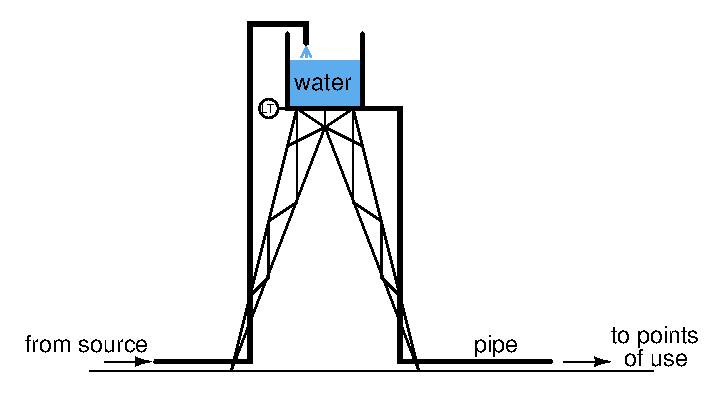
\includegraphics[width=15.5cm]{i00253x01.eps}$$

En trykkbasert nivåtransmitter står i dag ved bunnen av tanken, på toppen av tårnet, og måler vannnivå i tanken.  Den har kalibrert område 0 til 10 fot (0 til 120 inches W.C.).  Problemet er at vannet i transmitteren noen ganger fryser om vinteren, slik at nivåmålesystemet stopper.  Vannet i lagertanken og de store rørene fryser ikke, fordi sirkulasjonen fra forbruk holder temperaturen oppe.

Det besluttes å flytte transmitteren ned på bakkenivå ved foten av tårnet, slik at den kan stå i et lite oppvarmet hus og aldri fryse.  Ved å koble transmitteren direkte til det store vannrøret fra tanken til forbrukspunktene, kan hydrostatisk trykk fortsatt måles på dette punktet:

$$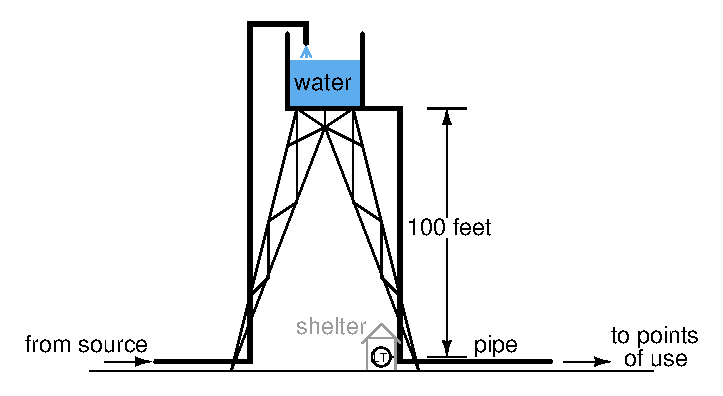
\includegraphics[width=15.5cm]{i00253x02.eps}$$

Beregn nye kalibreringspunkter (nedre og øvre måleverdi) for transmitteren i ny plassering.  Beregn også vannnivået i tanken når transmitterutgangen er 13.7 mA, samt hydrostatisk trykk på dette punktet i PSI.

\vskip 10pt

Angi til slutt om flyttingen ga skift i \textit{zero}, i \textit{span}, eller begge.

\underbar{file i00253}
%(END_QUESTION)





%(BEGIN_ANSWER)

Nedre måleverdi: 100 feet W.C. innsignal (1200 inches W.C.) = 4 mA utsignal

Øvre måleverdi: 110 feet W.C. innsignal (1320 inches W.C.) = 20 mA utsignal

\vskip 10pt

Vannnivå i tank ved 13.7 mA = 6.0625 fot ; påført trykk = 45.98 PSI

%(END_ANSWER)





%(BEGIN_NOTES)

Flyttingen av transmitteren til bunnen av tårnet ga et stort \textit{zero}-skift i kalibreringsområdet, men ingen endring i span.

\vskip 10pt

Jeg har selv flyttet en vannnivåtransmitter på akkurat denne måten: fra tårntopp til bakkenivå, og av samme grunn.  En utfordring var å finne en transmitter som kunne håndtere så stor nullpunktsundertrykking med så lite spenn.  Det avgjørende ved valg av transmittermodell var tilstrekkelig \textit{rangedown}: å kunne redusere spenn så mye samtidig som nullpunktsforskyvningen var stor.

Den opprinnelige transmitteren var en Rosemount 1151.  Jeg fikk ikke skrudd spennet langt nok ned på denne, og måtte bytte til en nyere Rosemount 3051, som da var relativt ny (midt på 1990-tallet).

%INDEX% Measurement, level: hydrostatic pressure
%INDEX% Process: water storage tank (elevated)

%(END_NOTES)
